\chapter{PROJETO}
\label{chp:projeto}

O projeto desta aplicação visa entregar um produto de software
desenvolvido de acordo com as necessidades da lista de discussão ``Rumo à
Certificação PHP'', a fim de auxiliar os profissionais que participam deste
grupo a gerenciar o banco de questões (perguntas/respostas) de maneira eficiente e,
além disto, disponibilizar uma ferramenta de simulado para que os profissionais 
possam utilizar durante os estudos para a prova de certificação \acs{ZCPE}
\cite{googleGroupsRumoACertificaoPHP}.

Desta forma, será possível ter um repositório de questões gerenciáveis. O
sistema proposto foi desenvolvido utilizando tecnologias livres, sendo 
que, foi escolhida a linguagem de programação \acs{PHP} e o
\textit{framework} \textit{Symfony 2} por conta da experiência e vivência do
autor nesta tecnologia e biblioteca respectivamente.

Também foram utilizadas as seguintes tecnologias livres: o banco de dados
relacional MySQL, a linguagem de marcação HTML, a linguagem de folhas de estilo 
em cascata CSS,  a linguagem de script do lado cliente (cliente-side) Javascript 
e a linguagem para manipulação dos dados no banco SQL.

Antes do projeto ser iniciado, houve uma pesquisa referente as ferramentas
semelhantes disponíveis no mercado, entretanto, como o foco da aplicação possui
requisitos de negócio específicos para o público alvo envolvido, o autor julgou
iniciar o projeto em uma nova plataforma, devendo esta ser: robusta (fornecendo
todo o suporte necessário para melhorias), livre (sem custos comerciais) e
principalmente que fosse do conhecimento do autor (por conta do tempo investido
em dominar uma nova plataforma tendo em vista o cronograma imposto pela
instituição de ensino).

Dentre as ferramentas estudadas, foi
verificada a \textit{SZES}, que utiliza como base o \textit{framework}
\textit{Silex}, mas, seu uso não foi adotado por conta desta aplicação
ter pretensões menores, por conta disto, para adaptar as demais funcionalidades
previstas seria necessário reestruturar a aplicação
base em um curto período de tempo, entretanto, esse foi o projeto que mais se
assemelhou aos objetivos da ferramenta proposta \cite{githubSZES}.

O projeto também conta com a implementação de interfaces simples, intuítivas e
fáceis de usar, que conforme afirma \citeonline{ergonomiaEUsabilidade}, permitem
que os usuários do software atinjam os seus objetivos com menos esforço,
trazendo benefícios para todos os \textit{stakeholders}. Entende-se a
importância da usabilidade, no entanto, sabendo que este trabalho não tem como
contribuição principal este recurso, não será detalhada a forma como as
interfaces foram desenvolvidas.

O projeto já encontra-se em uso e está sendo atualmente utilizado para 
gerenciar as perguntas do grupo de discussão e fornecer uma \ac{API} para que 
terceiros possam consumir os dados, entretanto, a funcionalidade que permite a
um profissional realizar um simulado ainda não está concluída. O código fonte da
aplicação está disponível em um repositório do \textit{GitHub} no seguinte
endereço \cite{githubZCPE}.

Com base na \acs{API} que foi desenvolvida, um participante da lista de
discussão se manifestou a fim de realizar a integração de sua aplicação móvel (para a
plataforma Android) com o repositório de perguntas e respostas através da arquitetura
\ac{REST}, disponível na \textit{Google Play} e intitulado como \textit{PHP ZCE
Practice Exam} \cite{googlePlayPHPZCEPracticeExam}.

\section{REQUISITOS}

A seguir será apresentado a especificação dos requisitos de software para a
ferramenta proposta, lembrando que, esses requisitos tiveram colaborações dos
próprios participantes da lista de discução ``Rumo a Certificação PHP''.

\begin{alineas}
	\item o sistema deverá ser desenvolvido com a linguagem PHP 5.4+;
	\item o sistema deverá persistir as informações em um base de dados relacional
	do MySQL 5;
	\item o sistema deverá rodar em uma infraestrutura em nuvem;
	\item o sistema irá ser executado em um navegador e o usuário deverá possuir
	conexão com a internet para poder acessar o sistema;
	\item o sistema deverá autenticar os usuários mediante usuário e senha ou
	conta Google, entretanto, os usuários que não estiverem autenticados poderão
	acessar o gerador de templates de e-mail e a área de login;
	\item para autenticação através de uma conta Google, o sistema deverá realizar
	a autenticação utilizando o protocolo \textit{OAuth2};
	\item o sistema deverá permitir que usuários sem conta de acesso e que não
	possuam ou não queiram utilizar uma conta Google, possam gerar templates de
	e-mail com o layout padrão de perguntas/respostas;
    \item o sistema deverá estar preparado para internacionalização, tendo como
    opções de idioma para o usuário final: o inglês e o português;
    \item assim que os usuários realizarem a autenticação, o sistema deverá
    exibir um \textit{dashboard} contendo um resumo sobre o gerenciamento das
    perguntas e respostas;
    \item haverão três papéis (tipos de conta no que diz respeito a permissão
    de acesso) de usuários dentro da aplicação, o usuário padrão, o usuário
    contribuidor e o super usuário;
    \item o sistema deverá redirecionar os usuário que não tiverem permissão a
    administração para a página inicial do projeto;
    \item o usuário padrão poderá gerenciar apenas as suas perguntas/respostas,
    listar as categorias e listar as tags;
    \item o usuário contribuidor terá os mesmos direitos do usuário padrão,
    porém, poderá adicionalmente gerenciar as perguntas e respostas de qualquer
    usuário;
    \item o super usuário poderá realizar qualquer procedimento do usuário
    contribuidor, e adicionalmente, gerenciar as categorias, tags, usuários e
    permissões de acesso;
    \item os usuários que se autenticarem com um usuário e senha poderão
    disparar e-mails (após cadastrar uma pergunta/resposta) para a lista de
    discussão pelo próprio sistema (através de uma conta SMTP do sistema);
    \item os usuários que se autenticarem com uma conta Google, além de disparar
    os e-mails via SMTP do sistema, poderão disparar os e-mails com a sua conta
    Google (através de uma integração da aplicação com a API fornecedia pelo
    Google Gmail);
    \item o sistema deverá gerenciar tags, que serão compostas por um título,
    sendo que, cada tag poderá ter uma ou várias questões associadas;
    \item o sistema deverá gerenciar categorias, que serão compostas por um
    título e uma descrição, sendo que, cada categoria poderá ter uma ou várias
    questões associadas e cada questão deverá ter ao menos uma categoria;
    \item o sistema deverá manter os seguintes tipos de respostas para o
    cadastro de perguntas: única escolha, múltipla escolha e texto aberto;
    \item o sistema deverá gerenciar as perguntas, que serão compostas por: id
    do grupo de discussão, tipo de questão (chave estrangeira),  autor da
    pergunta, enunciado e possíveis respostas (de acordo com o tipo de questão).
    Além disto, o sistema deverá manter campos de controle (\textit{booleanos})
    referente ao \textit{status} da pergunta, tais como: email foi enviado, a
    pergunta tem uma ou mais respostas corretas, aprovado, importado do google
    groups e revisado;
    \item a pergunta terá seu estado ``email foi enviado'' alterado quando o
    e-mail for disparado para o google groups pelo sistema, ou quando o sistema
    importar a pergunta do google groups sem que um usuário cadastre a questão
    manualmente;
    \item a pergunta terá seu estado ``pergunta tem uma ou mais respostas
    corretas'' alterado quando o usuário que estiver operando o sistema marcar
    uma ou mais respostas como corretas para a questão;
    \item a pergunta terá seu estado ``aprovado'' alterado quando o usuário com
    permissão administrativa configurar a pergunta como aprovada para ser
    exibida no simulado;
    \item a pergunta terá seu estado ``importado do google groups'' alterado
    quando o sistema importar a pergunta do google groups sem que haja um
    cadastro manual da pergunta por um usuário da aplicacação;
    \item a pergunta terá seu estado ``revisado'' alterado quando o usuário
    confirmar que a questão está pronta para ser utilizada pelo simulado ou
    publicada na lista de discussão;
    \item o sistema deverá permitir a exportação dos dados exibidos em ``xls''
    para permitir a manipulação da informação em planilhas do ``Excel'';
    \item o sistema deverá permitir que o usuário filtre todas as tags
    existentes por parte do título da tag;
    \item o sistema deverá permitir que o usuário filtre todas as categorias
    existentes por parte do título da categoria;
    \item o sistema deverá permitir que o usuário filtre todas as perguntas que
    foram: revisadas, aprovadas, email foi enviado, importado do google groups,
    além de permitir que o usuário informe o identificador único da pergunta, ou
    parte do enunciado da questão;
    \item o sistema deverá realizar um parser das informações presentes na lista
    de discussão com o objetivo de inserir as perguntas no sistema
    automaticamente, esta funcionalidade será necessária para a importação dos
    registros do google groups e também para os usuários que não tiverem ou não
    quiserem uma conta na aplicação;
    \item desenvolver o simulador de perguntas e respostas, sendo que, para
    realizar o simulado o usuário deverá estar autenticado no sistema com as
    suas credenciais;
    \item para iniciar o simulado, após realizar a autenticação, o usuário
    escolherá a quantidade de perguntas e que categorias de questões serão
    exibidas durante a sessão, sendo que, com base na quantidade de questões
    selecionadas o sistema irá criar um simulado com tempo para término
    proporcional a quantidade de questões;
    \item logo após a realização do simulado, o usuário deverá apresentar que 
    categoria de questões o participante teve menos acertos e com isso o
    candidato poderá focar seus estudos onde possui mais dificuldades;
    \item o layout da aplicação deverá ser responsivo, permitindo que o acesso
    seja realizado com dispositivos móveis;
    \item a plataforma deverá fornecer uma \acs{API} para consumir os dados do
    repositório de perguntas e respostas, facilitando a implementação de
    terceiros mediante autenticação.
\end{alineas}


\section{DIAGRAMA DE CASOS DE USO}

De acordo com \citeonline{umlGuiaDoUsuario}, um caso de uso especifica o
comportamento essencial de um sistema ou subsistema em uma visão macro, sem que
haja a implementação de tal funcionalidade, permitindo que, desenvolvedores, 
usuários e especialistas do domínio de negócio possam compreender as ações e 
papéis envolvidos no sistema, além disto, serve para a validação da arquitetura 
e da aplicação (ao decorrer da implementação do projeto de software). Na Figura
\ref{fig:diagramaCasosDeUso}, é apresentado diagrama de casos de uso da aplicação.

\begin{figure}[h!tb]
	\caption{Diagrama UML de Casos de Uso}
	\label{fig:diagramaCasosDeUso}

	\centering
	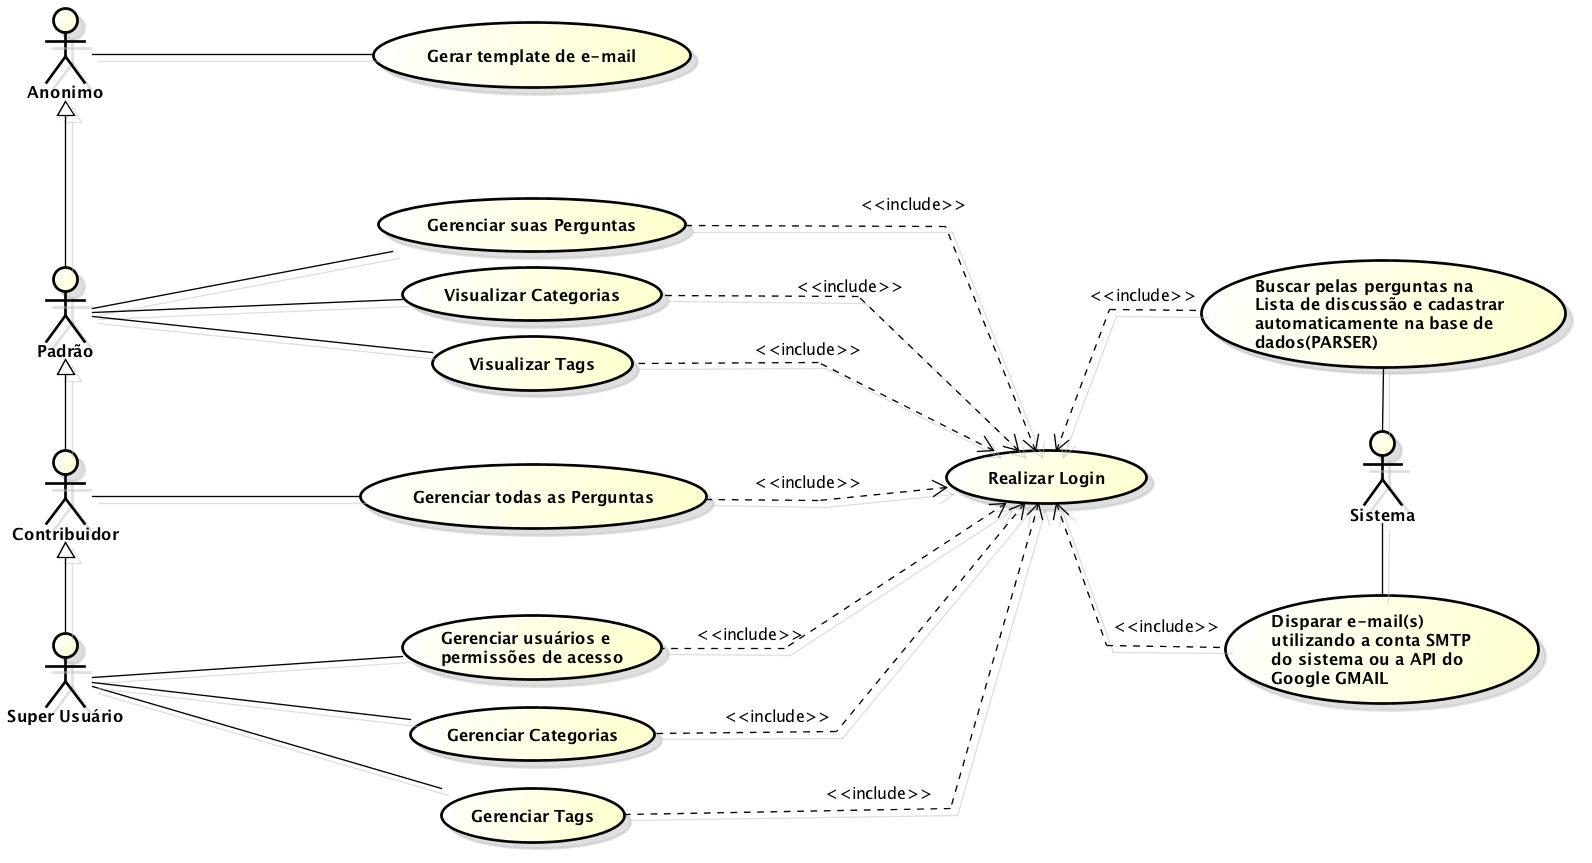
\includegraphics[width=\textwidth]{images/usecase.png}

	\centering
	\footnotesize Fonte: \fonteOAutor
\end{figure}

\FloatBarrier 	% Este comando impede que as imagens
				% flutuem a partir deste ponto no seu documento

\section{DIAGRAMA DE CLASSE}

Conforme afirma \citeonline{uml2RapidoEPraticoGuiaDeReferencia}, o diagrama de 
classe tem como objetivo agrupar comportamentos e estados em comum e definir 
relações estáticas do software, ou seja, ele descreve a arquitetura física dos 
componentes do sistema e de que forma eles estão organizados.


\section{MODELO ENTIDADE RELACIONAMENTO}

Na Figura \ref{fig:modeloEntidadeRelacionamento}, é apresentado a modelagem do
banco de dados.

\begin{figure}[h!tb]
	\caption{Modelo Entidade Relacionamento}
	\label{fig:modeloEntidadeRelacionamento}

	\centering
	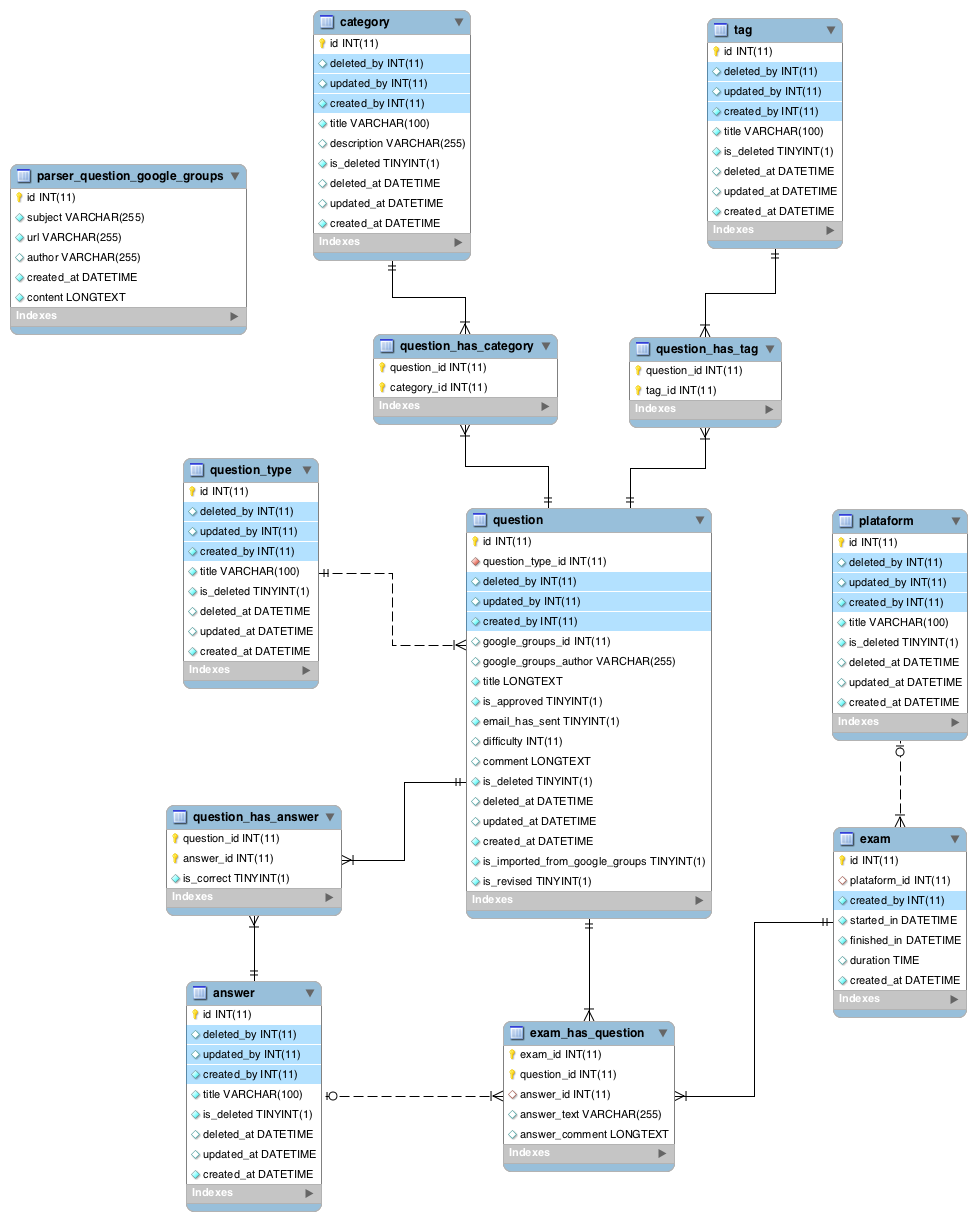
\includegraphics[width=\textwidth]{images/zcpe-reverse-engineer-database.png}

	\centering
	\footnotesize Fonte: \fonteOAutor
\end{figure}

\FloatBarrier 	% Este comando impede que as imagens
				% flutuem a partir deste ponto no seu documento

Viu-se neste capítulo as tecnologias utilizadas para a codificação da
ferramenta, a aplicação SZES (a que mais se assemelha aos objetivos propostos
por este trabalho), as definições dos requisitos funcionais e não funcionais, o
diagrama de casos de uso e o modelo do banco de dados. O capítulo a seguir 
apresenta os resultados obtidos com este projeto.
